%!TeX root = ./../Bachelorarbeit.tex

%##########################################################
% Inhalt
%##########################################################

\clearpage
\chapter{Konzeption}

\section{Auswahl der Peripherie}
\label{sec:concept-periphery-selection}

Für diese Arbeit wurde das \textit{\ac{gpio}} und das
\textit{\ac{uart}}-Peripheriemodul für Tests und Implementierung ausgewählt.
Beide Schnittstellen sind für eingebettete Systeme unerlässlich und können für
verschiedenste Anwendungen eingesetzt werden.
\newline
UART wurde ausgewählt, da der Aufwand der Integration bereits in QEMU
bestehender Schnittstellen bewertet werden soll.
Es existiert bereits eine Implementation eines UART Controllers für einen
Mikrocontroller der STM32F2-Familie.
Da Mikrocontroller Modelle der STM32F2 und STM32F4 Familien Pin-kompatibel
sind, sollte die bestehende Implementation des UART Controllers ebenfalls
für den STM32F429 SoC verwendet werden können.
Darüber hinaus ist die Funktionalität von UART im Vergleich zu anderen
seriellen Schnittstellen einfacher zu testen.
Es können Funktionen wie ARM's \textit{Semihosting} verwendet werden, um
beispielsweise durch UART übertragene Zeichen in der Kommandozeile auszugeben.
Dies verringert die Komplexität der Testprogramme, da keine speziellen
Änderungen für die jeweilige Testumgebung (QEMU oder echte Hardware)
erforderlich sind.
\newline
Die GPIO Schnittstelle wurde für eine neue, eigenständige Implementierung in
QEMU ausgewählt.
Sie weist eine vergleichsweise geringe Komplexität auf.
Testprogramme für die GPIO Funktionalität sollten ebenfalls ohne Anpassungen
sowohl in QEMU, als auch auf echter Hardware laufen.
In QEMU Version 9.0 existiert bereits eine Integration für einen
Mikrocontroller der STM32L4-Familie.
Das GPIO-Peripheriemodul der STM32L4-Familie ist allerdings nicht kompatibel
zum GPIO-Peripheriemodul der STM32F4-Familie.
Es verfügt über eine andere Anzahl an Peripherie Registern, mit anderen
Funktionalitäten.
Die Implementierung kann daher nur als Orientierung dienen und muss
entsprechend angepasst werden.

\section{QEMU Erweiterungen}

QEMU unterscheidet bei der Emulation von ARM Systemen zwischen Maschinen und
\ac{cpu}'s.
Die Maschine ist in der Regel ein spezielles Entwicklungsboard eines
Herstellers, welches einen \ac{soc} auf einer Leiterplatte integriert, zum
Beispiel das STM32F429-Discovery\cite{Stm32F429DiscoveryBoard} oder das
Olimex-STM32-E407\cite{OlimexStm32E407Board}.
\newline
In QEMU werden Maschine und SoC meist getrennt implementiert.
Die Maschine, bzw. das Entwicklungsboard, agiert dabei als Container für den
SoC.
Die meisten Funktionalitäten, sowie die Peripherie, werden im SoC
implementiert und der Maschine zur Verfügung gestellt.
Die CPU ist für die meisten \acp{soc} festgesetzt, da auf der echten Hardware
ebenfalls standardmäßig nur eine CPU zur Anwendung kommt.
Die CPU Architektur des STM32F429 Mikrocontrollers, \textit{Cortex-M4F} kann
vollständig in QEMU emuliert werden.
Beide der folgenden Ansätze sollen die CPU Emulation nutzen und um bestimmte
Peripherien erweitern.

\subsection{QEMU Device Implementierung} \label{konzept-qemu-dev}

Zunächst soll untersucht werden, wie eine Maschine und der dazugehörige SoC
direkt in QEMU integriert werden kann.
Das QEMU Projekt ist bereits über 20 Jahre alt und verfügt über diverse
\acp{api}.
Diese sollen genutzt werden, um das Projekt durch den STM32F429-\ac{soc} zu
erweitern.
Desweiteren soll eine Maschine integriert werden welche den \ac{soc}
implementiert.
Der grobe Ablauf dieser Erweiterung besteht also aus folgenden Abschnitten:
\begin{enumerate}
    \item Hinzufügen neuer Build-System Konfiguration für \ac{soc},
    \item Implementierung des STM32F429-\ac{soc},
    \item Integration bestehender Peripherie (\ac{uart}, SysCfg, etc.) in
        \ac{soc},
    \item Hinzufügen neuer Build-System Konfiguration für GPIO-Peripherie
    \item Implementierung der neuen Peripherie und Integration in \ac{soc}
\end{enumerate}
Die Adressen der Peripherie müssen dem Technischen-Referenzwerk des
STM32F429-Mikrocontrollers entnommen werden.
Die Funktionsweise und Konfiguration der Peripherie-Register sind dort
ebenfalls beschrieben.
Wie in Abbildung \ref{fig:QemuDeviceErweiterung} zu sehen ist, erstellt die
Maschine den \ac{soc}, welcher wiederum die konfigurierte Peripherie erstellt.
\begin{figure}[!htb]
    \centering
    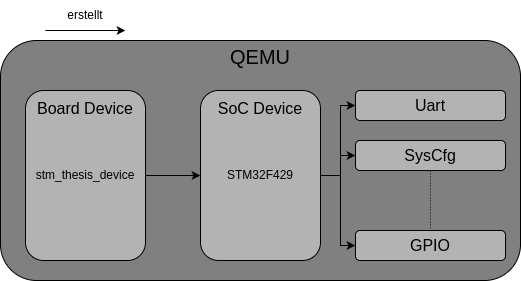
\includegraphics[width=0.7\textwidth]{anlagen/bilder/Qemu_Device}
    \caption{Grobe Skizzierung der Interaktion zwischen Maschine, \ac{soc} und Peripherie}
    \label{fig:QemuDeviceErweiterung}
\end{figure}


\subsection{External Device Interface Implementierung}

Im zweiten Ansatz soll ein weiteres Konzept für die Integration neuer
\ac{soc}'s in QEMU vorgestellt werden.
Bei dieser Methode wird die Implementierung der Peripherie in externe Prozesse
verlagert.
Die Unterscheidung zwischen CPU und Maschine besteht zwar auch bei diesem
Ansatz, allerdings ist der Funktionsumfang der Maschine stark reduziert, da sie
keine Peripherie direkt über den \ac{soc} integriert.
Die Maschine agiert hier nur als generischer Container, welcher Verbindungen
entgegennimmt.
Im Gegensatz zum ersten Ansatz muss nicht für jeden neuen Mikrocontroller eine
separate Maschine mitsamt \ac{cpu} implementiert werden.
Die relevanten Schnittstellen laufen jeweils gekapselt in einem separaten
Prozess.
Wie in Abbildung \ref{fig:QemuExternalDeviceErweiterung} zu sehen ist,
kommunizieren der \ac{soc} und Peripherie mittels \ac{ipc}.
\begin{figure}[!htb]
    \centering
    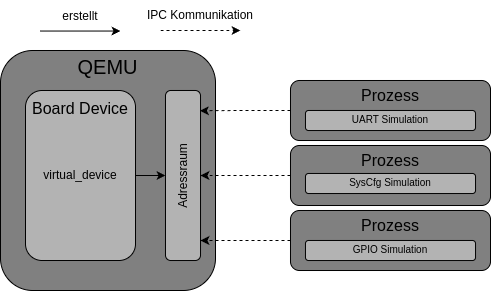
\includegraphics[width=0.7\textwidth]{anlagen/bilder/Qemu_external_device}
    \caption{Grobe Skizzierung der Interaktion zwischen QEMU und externen Prozessen}
    \label{fig:QemuExternalDeviceErweiterung}
\end{figure}
Dies ermöglicht eine unabhängige Implementierung von Peripherie und \ac{soc}.
Die Interprozesskommunikation wird mittels der externen Bibliothek
\textit{nanomsg} realisiert, welche in den QEMU Event-Loop integriert
wurde\cite{NanoMsg}.
Die Verbindung von QEMU-Emulation und den separaten Prozessen erfolgt bei Start
der QEMU-Anwendung.
Dort können einzelne Devices oder eine Gruppe von Devices mit einer
spezifischen Adresse im Adressraum des \ac{soc} verbunden werden.
Die Konfiguration des \ac{soc} erfolgt ebenfalls bei Start der QEMU Anwendung.
Die Integration der Erweiterung existiert bereits in einem separaten
Repository\cite{QemuEdiRepo}.
Dieses soll genutzt werden, um die QEMU Anwendung zu bauen.
\newline
Im Gegensatz zum ersten Ansatz kann eine Testanwendung die das \ac{edi}
implementiert nicht unverändert sowohl in QEMU als auch auf realer Hardware
laufen.
Hierfür wird eine weitere Abstraktionsschicht benötigt, welche die Aufrufe an
die Peripherie abfängt und entsprechend der Umgebung behandelt.
Im Rahmen des Vortrags wurde eine Demo-Applikation vorgestellt, welche das
\textit{CMake} Build-System nutzt, um die Anwendungen für QEMU und Hardware zu
implementieren\cite{EdiDemoRepo}.
Um die Komplexität möglichst gering zu halten soll versucht werden, die
Demo-Applikation auf den STM32F429-\ac{soc} anzuwenden.
Das Testprogramm für die reale Hardware greift auf die externe, quelloffene
Bibliothek \textit{libopencm3}\cite{LibOpenCm3} zurück.
Da sowohl die Projektstruktur, als auch die Bibliothek nicht Teil der normalen
Testanwendungen sind, soll der Fokus auf der Interakton zwischen Anwendung 
und QEMU liegen.

\section{Testprogramme und Teststrategie}
\label{sec:concept-tests}

Um die korrekte Funktionsweise der Peripherie und \ac{soc} Implementierungen zu
testen, sollen verschiedene Testprogramme entwickelt werden.
Diese Testprogramme werden anschließend sowohl in QEMU als auch auf realer
Hardware ausgeführt.
Mögliche Unterschiede bei beiden Varianten sollen wärend der Ausführung
identifiziert werden.
Dabei wird sich auf den STM32F429-\ac{soc} mit der Cortex-M4 \ac{cpu}
beschränkt.
Während der Ausführung können unterschiedliche Verhalten in der Software für
emulierte und reale Umgebung auftreten.
Um diese gering zu halten, sollen die Testprogramme einfach gehalten werden.
\newline
Für die Entwicklung der Tests sollen ausschließlich die notwendigsten externen
Bibliotheken genutzt und konfiguriert werden.
Dies umfasst die STM-\textit{\ac{hal}}, für Programmierung und Konfiguration
der Peripherie.
Eine einheitliche Nutzung von Bibliotheken verringert ebenfalls den
Implementationsaufwand.
Zur Konfiguration der \ac{cpu} spezifischen Einstellungen soll das
\textit{\ac{cmsis}} verwendet werden.
Die eigentliche Testanwendung wird in \textit{C} programmiert.
Für die Testprojekte wird das Build-System \textit{Meson} verwendet, da dies
auch im QEMU Projekt zum Einsatz kommt und somit keine erneute Umgewöhnung
erfordert.
Sofern möglich soll auf quelloffene Anwendungen zurückgegriffen werden.
Die Entwicklungsumgebung sollte einfach gehalten werden, um leicht
reproduzierbar zu sein.
